El motor seleccionado será el\cite{EMG30datasheet} Por haber trabajado ya también con él.

\begin{figure}[H]
    \centering
    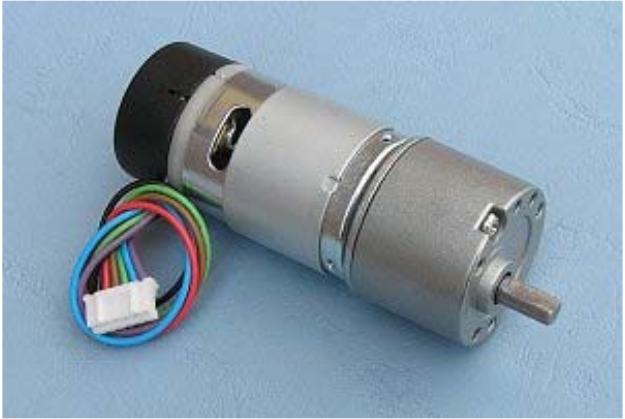
\includegraphics[scale = 0.4]{part/Proyecto_ejecutivo/memoria_constructiva/motor/img/MotorEMG30}
    \caption[Motor EMG30]{Motor EMG30\cite{EMG30datasheet}}\label{fig:EMG Motor}
\end{figure}

A continuación se muestran las características más relevantes del motor:

\begin{table}[H]
    \centering
    \begin{tabular}{|l|l|}
        \hline
        Característica & Valor\\
        \hline
        Voltaje nominal & 12 V\\
        \hline
        Torque nominal & 1.5 kg/cm\\
        \hline
        Velocidad nominal & 170 rpm\\
        \hline
        Intensidad nominal & 530 mA\\
        \hline
        Velocidad sin carga& 216 rpm\\
        \hline
        Intensidad sin carga& 150mA\\
        \hline
        Intensidad máxima& 2.5 A\\
        \hline
        Salidad nominal & 4.22 W\\
        \hline
        Pasos por vuelta del codificador& 360 \\
        \hline
        Razón de la reductora & 30:1\\
        \hline
    \end{tabular}
    \caption[Características EMG30]{Características EMG30 \\ Fuente:\cite{EMG30datasheet}}\label{tab:características EMG30}
\end{table}

El código de colores de las conexiones del motor podemos encontralo en las especificaciones ténicas del mismo
\begin{figure}[H]
    \centering
    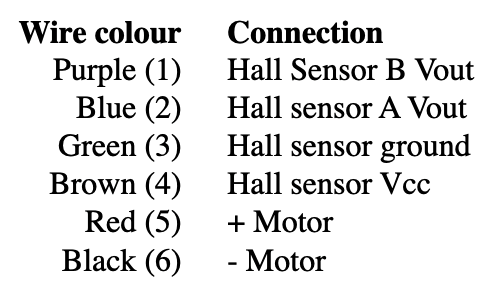
\includegraphics[scale = 0.6]{part/Proyecto_ejecutivo/memoria_constructiva/motor/img/motorConnection}
    \caption[Motor EMG30]{Motor EMG30 \\Fuente: Documento de especificaciones técnicas.\cite{EMG30datasheet}}\label{fig:motor connection}
\end{figure}

